\begin{frame}
	\frametitle{Kalman Filter}
	\note{información extraida de https://youtu.be/PiCC-SxWlH8}
	
	\begin{itemize}
		\item Es un Filtro de Bayes
		\item Todo es Gaussiano
		\begin{equation*}
			p(x)=\det(2\pi\covariance)^{\frac{1}{2}} \exp\left(-\dfrac{1}{2} (x - \mu )^{\top} \inverse{\covariance} (x - \mu )  \right)
		\end{equation*}
		
		\item Soluciones optimas para modelos lineales y distribuciones Gaussianas.
	\end{itemize}

	\begin{figure}[!h]
		\centering
		\subfloat[]
		{
			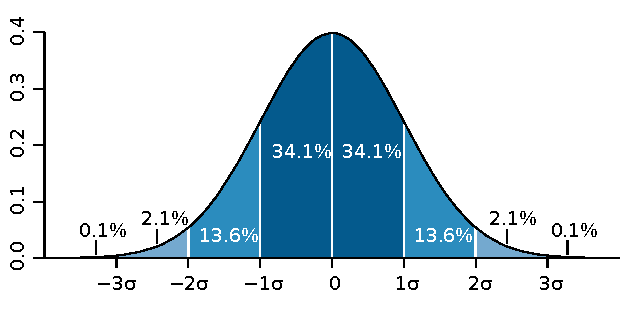
\includegraphics[width=0.3\columnwidth]{./images/standard_deviation_diagram.pdf}
		}
		\subfloat[AGREGAR ELIPSE ELIPSOIDE ]
		{
			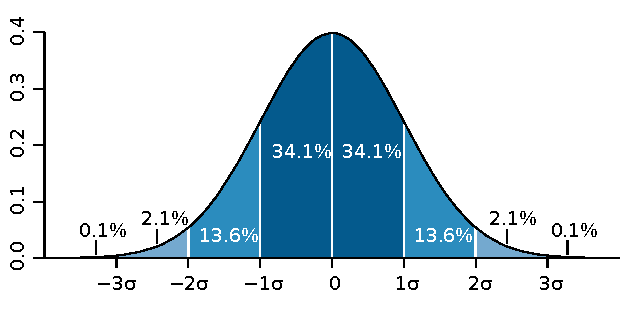
\includegraphics[width=0.3\columnwidth]{./images/standard_deviation_diagram.pdf}
		}
	\end{figure}
\end{frame}


\begin{frame}
	\frametitle{Kalman Filter Asunciones}
	\note{información extraida de https://youtu.be/PiCC-SxWlH8}
	
	\begin{itemize}
		\item Ruido y distribuciones Gaussianas
		\item Modelos de movimiento y observación lineales
	\end{itemize}

	\begin{align*}
		\state_{t} &= A_{t} \state_{t-1} + B_{t}\controlCommand_{t} + \motionModelNoise_{t}\\
		\observation_{t} &= C_{t} \state_{t} + \measurementModelNoise_{t}
	\end{align*}
	\note{Kalman Filter requiere que los ruidos sean gaussianos y que el estado resulte de una combinación lineal.}

	\centering
	\alert{¿qué pasa si este estas asunciones no pasan?}
	\note{Differencial drive y Ackerman motion models NO son modelos lineales}
	\note{Los observation models de un láser  o de una cámara tampoco son lineales.}
\end{frame}

\begin{frame}
	\frametitle{Sistemas dinámicos no Non-lineales}
	\note{información extraida de https://youtu.be/PiCC-SxWlH8}
	\begin{itemize}
		\item Los problemas reales en general emplean funciones no-lineales
	\end{itemize}
	
	\begin{align*}
		\state_{t} &= A_{t} \state_{t-1} + B_{t}\controlCommand_{t} + \motionModelNoise_{t}\\
		\observation_{t} &= C_{t} \state_{t} + \measurementModelNoise_{t}
	\end{align*}

\TODO{tachar las formulas lineales}

	\begin{align*}
		\state_{t} &= \motionModelFunction{\controlCommand_{t}, \state_{t-1}} + \motionModelNoise_{t}\\
		\observation_{t} &= \observationModelFunction{\state_{t}} + \measurementModelNoise_{t}
	\end{align*}

\end{frame}

\begin{frame}
	\frametitle{Modelo de movimiento linearizado}
	\note{información extraida de https://youtu.be/PiCC-SxWlH8}
	
	\begin{itemize}
		\item Linearizar el modelo esta dado por:
	\begin{align*}
		p(\state_{t} | \controlCommand_{t}, \state_{t-1}) &\approx \det(2 \pi \motionModelCovariance_{t})^{\frac{1}{2}}\\
		&\exp (-\dfrac{1}{2} (\state_{t} - \motionModelFunction{\controlCommand_{t}-\mu_{t-1}} - \motionModelJacobian_{t}(\state_{t-1}-\mu_{t-1}))^{\top}\\
		&\inverse{\motionModelCovariance_{t}} (\state_{t} - \underbrace{\motionModelFunction{\controlCommand_{t},\mu_{t-1}} - \motionModelJacobian_{t} (\state_{t-1}-\mu_{t-1})}_{\text{modelo linearizado}}))
	\end{align*}
	
	\item $\motionModelCovariance_{t}$ describe el ruido del movimiento
	\end{itemize}	
\end{frame}

\begin{frame}
	\frametitle{Modelo de observación linearizado}
	\note{información extraida de https://youtu.be/PiCC-SxWlH8}
	
	\begin{itemize}
		\item Linearizar el modelo esta dado por:
		\begin{align*}
			p(\observation_{t} | \state_{t}) &\approx \det(2 \pi \observationModelCovariance_{t})^{\frac{1}{2}}\\
			&\exp (-\dfrac{1}{2} (\observation_{t} - \observationModelFunction{\overline{\mu_{t}}} - \observationModelJacobian_{t}(\state_{t} - \overline{\mu_{t}}))^{\top}\\
			&\inverse{\observationModelCovariance_{t}} (\observation_{t} - \underbrace{\observationModelFunction{\overline{\mu_{t}}} - \observationModelJacobian_{t} (\state_{t}-\overline{\mu_{t}})}_{\text{modelo linearizado}}))
		\end{align*}
		
		\item $\observationModelCovariance_{t}$ describe el ruido de la medición
	\end{itemize}	
	
	
\end{frame}

\begin{frame}
	\frametitle{Algoritmo de Filtro de Kalman Extendido}
	\note{información extraída de https://youtu.be/PiCC-SxWlH8}
	
    \begin{algorithmic}[1]
    \Procedure{ExtendedKalmanFilter}{$\mu_{t-1}, \covariance_{t-1}, \controlCommand_{t}, \observation_{t}$}
        \State $\overline{\mu}_{t} = \motionModelFunction{\controlCommand_{t}, \mu_{t-1}}$
        \State $\overline{\covariance}_{t} = \motionModelJacobian_{t} \covariance_{t-1} \motionModelJacobian_{t}^{\top}+\motionModelCovariance_{t}$
        \Statex
        \State $\kalmanGain_{t} = \overline{\covariance}_{t} \observationModelJacobian_{t}^{\top} (\observationModelJacobian_{t} \overline{\covariance}_{t}  \observationModelJacobian_{t} + \observationModelCovariance_{t})^{-1} $
        \State $\mu_{t} = \overline{\mu}_{t} + \kalmanGain_{t} (\observation_{t} - \observationModelFunction{\overline{\mu}_{t}})$
        \State $\covariance_{t} =  (I - \kalmanGain_{t} \observationModelJacobian_{t}) \overline{\covariance}_{t}$
        \State \Return $\mu_{t}, \covariance_{t}$
    \EndProcedure
    \end{algorithmic}
\end{frame}

\section{EKF Localización for feature-based map}

\begin{frame}
	\frametitle{Odometry as controls}
	\note{información extraida de https://youtu.be/PiCC-SxWlH8}
	
   	\begin{figure}[!h]
        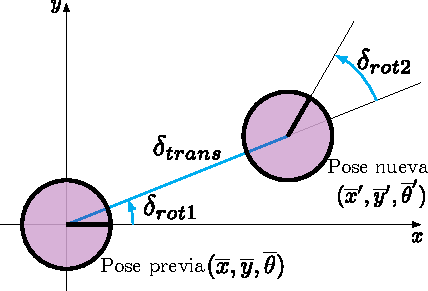
\includegraphics[width=0.6\columnwidth]{./images/odometry_as_controls.pdf}
    \end{figure}

    \begin{equation*}
        \controlCommand = (\delta_{rot1}, \delta_{trans}, \delta_{rot2})
    \end{equation*}
	
\end{frame}

\begin{frame}
	\frametitle{Motion model}
	\note{información extraida de https://youtu.be/PiCC-SxWlH8}
	
	\begin{itemize}
		\item Odometría de modelo de movimiento
		\begin{equation*}
			\begin{bmatrix}
				x^{\prime} \\
				y^{\prime} \\
				\theta^{\prime}
			\end{bmatrix} =
			\underbrace{
				\begin{bmatrix}
				x \\
				y \\
				\theta
			\end{bmatrix} +
			\begin{bmatrix}
				\delta_{trans}\cos(\theta+\delta_{rot_{1}}) \\
				\delta_{trans}\cos(\theta+\delta_{rot_{1}}) \\
				\delta_{rot_{1}} + \delta_{rot_{2}}
			\end{bmatrix}
			}_{\motionModelFunction{\controlCommand_{t}, \state_{t-1}}} + \normalDistribution{0}{\motionModelCovariance_{t}}
		\end{equation*}
		\item Linearización
		\begin{equation*}
			\motionModelFunction{\controlCommand_{t}, \state_{t-1}} \approx 			\motionModelFunction{\controlCommand_{t}, \mu_{t-1}} + \covariance_{t}(\state_{t-1}-\mu_{t-1})
		\end{equation*}
	\end{itemize}
	
\end{frame}

\begin{frame}
	\frametitle{Jacobianos del modelo de movimiento}
	\note{información extraida de https://youtu.be/PiCC-SxWlH8}
	Calculamos el Jacobiano con respecto al estado
	\begin{equation*}
		\motionModelJacobian_{t} = \dfrac{\delta\motionModelFunction{\controlCommand_{t},\mu_{t-1}}}{\delta \state_{t-1}} =
		\begin{bmatrix}
			\dfrac{\delta x^{\prime}}{\delta \mu_{t-1,x}} & \dfrac{\delta x^{\prime}}{\delta \mu_{t-1,y}} & \dfrac{\delta x^{\prime}}{\delta \mu_{t-1,\theta}}\\
			\dfrac{\delta y^{\prime}}{\delta \mu_{t-1,x}} & \dfrac{\delta y^{\prime}}{\delta \mu_{t-1,y}} & \dfrac{\delta y^{\prime}}{\delta \mu_{t-1,\theta}}\\
			\dfrac{\delta \theta^{\prime}}{\delta \mu_{t-1,x}} & \dfrac{\delta \theta^{\prime}}{\delta \mu_{t-1,y}} & \dfrac{\delta \theta^{\prime}}{\delta \mu_{t-1,\theta}}\\
		\end{bmatrix}
	\end{equation*}

	\begin{equation*}
	\motionModelJacobian_{t} = 
	\begin{bmatrix}
		1 & 0 & -\delta_{trans} \sin(\theta + \delta_{rot_{1}})\\
		0 & 1 & \delta_{trans} \cos(\theta + \delta_{rot_{1}})\\
		0 & 0 & 1\\
	\end{bmatrix}
	\end{equation*}
\end{frame}

\begin{frame}
	\frametitle{Jacobianos del modelo de movimiento}
	\note{información extraida de https://youtu.be/PiCC-SxWlH8}
	Calculamos el Jacobiano con respecto al comando de control
	\begin{equation*}
		\motionModelJacobianControl{t} = \dfrac{\delta\motionModelFunction{\controlCommand_{t},\mu_{t-1}}}{\delta \controlCommand_{t}} =
		\begin{bmatrix}
			\dfrac{\delta x^{\prime}}{\delta \controlCommand_{t,\delta_{rot_{1}}}} & \dfrac{\delta x^{\prime}}{\delta \controlCommand_{t,\delta_{trans}}} & \dfrac{\delta x^{\prime}}{\delta \controlCommand_{t,\delta_{rot_{2}}}}\\
			\dfrac{\delta y^{\prime}}{\delta \controlCommand_{t,\delta_{rot_{1}}}} & \dfrac{\delta y^{\prime}}{\delta \controlCommand_{t,\delta_{trans}}} & \dfrac{\delta y^{\prime}}{\delta \controlCommand_{t,\delta_{rot_{2}}}}\\
			\dfrac{\delta \theta^{\prime}}{\delta \controlCommand_{t,\delta_{rot_{1}}}} & \dfrac{\delta \theta^{\prime}}{\delta \controlCommand_{t,\delta_{trans}}} & \dfrac{\delta \theta^{\prime}}{\delta \controlCommand_{t,\delta_{rot_{2}}}}
		\end{bmatrix}
	\end{equation*}
	
	\begin{equation*}
		\motionModelJacobianControl_{t} = 
		\begin{bmatrix}
			-\delta_{trans} \sin(\theta + \delta_{rot_{1}}) & \cos(\theta + \delta_{rot_{1}}) & 0\\
			\delta_{trans} \cos(\theta + \delta_{rot_{1}}) & \sin(\theta + \delta_{rot_{1}}) & 0\\
			0 & 0 & 1\\
		\end{bmatrix}
	\end{equation*}
\end{frame}

\begin{frame}
	\frametitle{Observation model}
	\note{información extraida de https://youtu.be/PiCC-SxWlH8}
		Calculamos el Jacobiano
	\begin{equation*}
		\motionModelJacobian_{t} = \dfrac{\delta\motionModelFunction{\controlCommand_{t},\mu_{t-1}}}{\delta \state_{t-1}} =
		\begin{bmatrix}
			\dfrac{\delta x^{\prime}}{\delta \mu_{t-1,x}} & \dfrac{\delta x^{\prime}}{\delta \mu_{t-1,y}} & \dfrac{\delta x^{\prime}}{\delta \mu_{t-1,z}}\\
			\dfrac{\delta y^{\prime}}{\delta \mu_{t-1,x}} & \dfrac{\delta y^{\prime}}{\delta \mu_{t-1,y}} & \dfrac{\delta y^{\prime}}{\delta \mu_{t-1,z}}\\
			\dfrac{\delta z^{\prime}}{\delta \mu_{t-1,x}} & \dfrac{\delta z^{\prime}}{\delta \mu_{t-1,y}} & \dfrac{\delta z^{\prime}}{\delta \mu_{t-1,z}}\\
		\end{bmatrix}
	\end{equation*}
	
	\begin{equation*}
		\motionModelJacobian_{t} = 
		\begin{bmatrix}
			1 & 0 & -\delta_{trans} \sin(\theta + \delta_{rot_{1}})\\
			0 & 1 & \delta_{trans} \cos(\theta + \delta_{rot_{1}})\\
			0 & 0 & 1\\
		\end{bmatrix}
	\end{equation*}
	
\end{frame}

\begin{frame}
	\frametitle{Jacobianos del observation model}
	\note{información extraida de https://youtu.be/PiCC-SxWlH8}
	
	
\end{frame}

\begin{frame}
	\frametitle{Algoritmo de Filtro de Kalman Extendido}
	\note{información extraida de https://youtu.be/PiCC-SxWlH8}
	
	
\end{frame}

\begin{frame}
	\frametitle{Algoritmo de Filtro de Kalman Extendido}
	\note{información extraida de https://youtu.be/PiCC-SxWlH8}
	
	
\end{frame}

\begin{frame}
	\frametitle{Prediction step}
	\note{información extraida de https://youtu.be/PiCC-SxWlH8}
	
	
\end{frame}

\begin{frame}
	\frametitle{Algoritmo de Filtro de Kalman Extendido}
	\note{información extraida de https://youtu.be/PiCC-SxWlH8}
	
	
\end{frame}

\begin{frame}
	\frametitle{Medición esperada}
	\note{información extraida de https://youtu.be/PiCC-SxWlH8}
	
\end{frame}

\begin{frame}
	\frametitle{Correction step}
	\note{información extraida de https://youtu.be/PiCC-SxWlH8}
	
\end{frame}

\begin{frame}
	\frametitle{2D EKF Localization Ejemplo}
	\note{información extraida de https://youtu.be/PiCC-SxWlH8}
	
\end{frame}

\begin{frame}
	\frametitle{EKF resumen}
	\note{información extraida de https://youtu.be/PiCC-SxWlH8}
	
\end{frame}

